%%%%%%%%%%%%%%%%%%%%%%%%%%%%%%%%%%%%%%%%%%%%%%%%%%%%%%%%%%%%%%%%%%%%%%%
%% Related Work
\subsection{Kinematik }
\label{sec:basics-ik}
    
Dieses Unterkapitel befasst sich mit dem Begriff der Kinematik und den dazu gehörigen Begriffen des Mechanismus und der inversen Kinematik. Außerdem werden einige mathematische Lösungswege für verschiedene Probleme innerhalb der dieser Themen genannt. Die folgenden Definitionen sind aus dem Buch \cite[Kapitel 7]{Corke2011} übernommen.

\subsubsection{Mechanismus}

Ein Mechanismus ist der Grundbegriff von beweglichen Körper. Dabei wird zwischen \textit{Gliedern} (engl. Link, $L$ = Set of Links) und \textit{Gelenken} (engl. Joint, $J$ = Set of Joints) unterschieden. Glieder sind die starren Körper eines Mechanismus und sind durch Gelenke miteinander verbunden. Ein Glied ist nicht auf ein Gelenk beschränkt, sondern kann mehrere haben ($N_{joint} \in \mathds{N}_0$). Auch die Verbindung zwischen zwei Gliedern kann durch mehrere  Gelenke realisiert sein. Ein Gelenk wiederum ist auf genau zwei Glieder beschränkt  ($N_{link} = 2$) und ermöglicht so eine eingeschränkte relative Bewegung zueinander. Gelenke werden nicht als eigenständige physikalische Körper gesehen. Gelenkhälften, zum Beispiel die Schenkel eines Kippscharniers, werden als Bestandteil des damit verbundenen Gliedes betrachtet. Die folgenden Definitionen sind als Denavit–Hartenberg Parameter bekannt \citep{Corke2011}.

Glieder können mit zwei Parametern definiert werden, der Länge $a$ und der Verdrehung $\alpha$:

\begin{displaymath}
	l_i \in L \\
\end{displaymath}

\begin{equation}
a_i =  \text{Länge von } l_i
\end{equation}

\begin{equation}
\alpha_i =  \text{Verdrehung von } l_i 
\end{equation}

Gelenke werden ebenfalls mit zwei Parametern definiert. Der Gelenk-Offset beschreibt den Abstand zwischen den zwei Gliedern eines Gelenks auf der Gelenkachse. Der Gelenkwinkel beschreibt die Rotation zwischen den beiden verbundenen Glieder im Bezug zur Gelenkachse\citep{Corke2011}.  Zur Veranschaulichung dieser Nomenklatur ist die Abbildung \ref{fig:ik-dh} vorhanden. Dabei sind die Parameter in rot dargestellt. Außerdem werden die einzelnen Koordinatensysteme der Gelenke gezeigt.

\begin{displaymath}
j_i \in J \\
\end{displaymath}

\begin{equation}
d_i =  \text{Gelenk-Offset von } j_i
\end{equation}

\begin{equation}
\theta_i =  \text{Gelenkwinkel von } j_i 
\end{equation}

\begin{figure}[H]
	\centering
	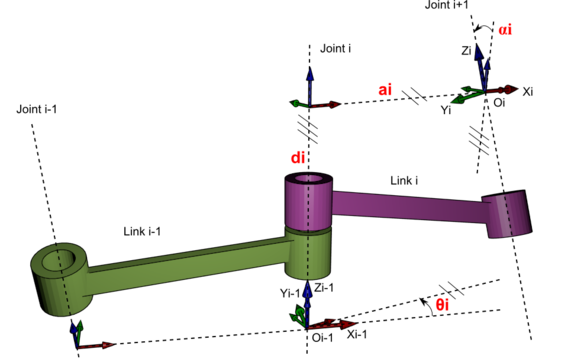
\includegraphics[width=0.8\textwidth]{fig/dh}   
	\caption[Darstellung Denavit–Hartenberg Parameter]{Darstellung Denavit–Hartenberg Parameter. Bildquelle \cite{wiki}}
	\label{fig:ik-dh}
\end{figure}

\subsubsection{Kinematik}
\label{sec:basics-ik-k}

Die \textit{Kinematik} eines Mechanismus beschreibt die Bewegungsmöglichkeiten der Glieder relativ zueinander. Es wird dabei abstrahiert, ob ein Gelenk motorisch angetrieben oder passiv bewegt wird. Die Kinematik betrachtet bei der Bewegung auftretende \textit{Geschwindigkeiten} und \textit{Beschleunigungen}. Auftretende Kräfte werden nicht in der Kinematik, sondern in der \textit{Dynamik} untersucht. Zentrale Aspekte dabei sind die Trägheits- und Schwerkraft.

Die \textit{Kinematische Kette} beschreibt den Aufbau eines speziellen Mechanismus. Dabei ist die Anzahl der Gelenke pro Glied auf maximal 2 beschränkt ($N_{joint} <= 2$). Besitzt jedes Glied genau zwei Gelenke gilt die Kette als geschlossen, ansonsten als offen:

\begin{equation}
	 \text{Kinematische Kette} = 
	\begin{cases}
		geschlossen & \forall l \in L | l_{joints} = 2 \\
		offen & \text{für Rest} \\
	\end{cases}
\end{equation}

Für diese Arbeit ist nur die offene Kette interessant, da die Manipulatoren der meisten Roboter an beiden Enden (Base und End-Effektor) frei sind. Dadurch ergibt sich für $N_{link} = N_{joint} + 1$. Typischerweise wird das erste Gelenk mit dem Index 1 versehen und das erste Glied mit dem Index 0. Glied 0 ist die \textit{Base} des Manipulators und Glied N beinhaltet den \textit{End-Effektor}. Aus der Bezeichnung ergibt sich, dass Gelenk j die Glieder j-1 und j mit einander verbindet und das Glied j bewegt \citep{Corke2011}. 

Die Transformation eines Glied-Koordinatensystems {j-1} zu Glied {j} wird durch elementare Rotation und Translation beschrieben (siehe auch Abbildung \ref{fig:ik-dh}):

\begin{equation}
^{j-1}A_{j}(\theta_j,d_j,a_j,\alpha_j) = T_{Rz}(\theta_j)T_{z}(d_j)T_{x}(a_j)T_{Rx}(\alpha_j)
\label{f:basics-ik-k}
\end{equation}


Durch die Vereinigung der einzelnen Matrizen ergibt sich \citep{Corke2011}:
\begin{equation}
^{j-1}A_{j}(\theta_j,d_j,a_j,\alpha_j) = 
\begin{pmatrix}
cos \theta_j & -sin \theta_j cos \alpha_j & sin \theta_j sin \alpha_j  & a_j cos \theta_j\\
sin \theta_j & cos \theta_j cos \alpha_j & -cos \theta_j sin \alpha_j  & a_j sin\theta_j\\
0 			&sin \alpha_j 				& cos \alpha_j  & d_j\\
0 & 0 & 0& 1\\
\end{pmatrix}
\end{equation}

\subsubsection{Forward Kinematics}

Die Vorwärts-Kinematik (engl. Forward Kinematic) beschreibt die "vorwärts"  Rechnung der Kinematik. Aus den gegebenen Gelenk-Informationen wird die Pose des End-Effectors $\xi_E$ berechnet. Hier reichen die Daten für den Gelenkwinkel $\theta_j$ bei Drehgelenken und für den Winkel-Offset $d_j$ bei Schiebe-/ Schubgelenken, da die restlichen Werte für den Mechanismus als konstant angesehen werden können. Die Forward Kinematic wird häufig als Funktion $K$ angegeben \citep{Corke2011}:

\begin{equation}
\xi_E = K(\textbf{q})
\label{f1}
\end{equation}

$q$ entspricht dabei der aktuellen Gelenk-Konfiguration und $\xi_E$ der Pose des End-Effectors. Durch die Kombination der Transformation aus Gleichung \ref{f:basics-ik-k} ergibt sich für einen Manipulator mit N-Gelenken  \citep{Corke2011}. Dies wird benötigt, um die aktuelle Pose des End-Effektors für den Roboter zu berechnen. In dem Anwendungsszenario für diese Arbeit wird dies unter anderem für Positionsüberprüfungen und Kollisionskontrollen, aber auch für die Übergabe benötigt.

\begin{equation}
\xi_E \sim \: ^0T_E =\: ^0A_1\:^1A_2 \:\dots\:^{N-1}A_N
\end{equation}

\subsubsection{Inverse Kinematik}

Die Inverse Kinematik berechnet die Inverse der Forward-Kinematic. Sie bestimmt die möglichen Gelenk-Konfigurationen $\textbf{q}$ für eine Zielpose. Im Gegensatz zur Forward-Kinematic ist die Inverse Kinematik nicht eindeutig. Eine einfache Veranschaulichung kann man am menschlichen Körper sehen. Fixiert man das Handgelenk an einer Position kann man den Ellenbogen in verschiedene Positionen bewegen, ohne die Position der Schulter zu ändern. Für die Inverse Kinematik ergibt sich folgende Funktion für eine beliebige Pose $\xi$ \citep{Corke2011}:


\begin{equation}
\textbf{q} = K^{-1}(\xi)
\label{f2}
\end{equation}

Aus Gleichung \ref{f1} und \ref{f2} ergibt sich auf Grund der Eindeutigkeit:

\begin{displaymath}
\xi = K(K^{-1}(\xi))
\end{displaymath}

Aber \textbf{nicht}
\begin{displaymath}
\textbf{q} = K^{-1}(K(\textbf{q}))
\end{displaymath}

Um eine Inverse Kinematik zu lösen gibt es drei Methoden: geometrisch (analytisch), numerisch und heuristisch \citep{danielasteidl2011}.

Die geometrische Lösung nutzt die einfache geometrische Abstraktion des Mechanismus und versucht diesen mit trigonometrischen Funktionen abzubilden. Damit auch hier mehrere Lösungen bestimmt werden können, werden verschiedene Konfigurationen für bestimmte Abstraktionsmodelle geschaffen und alle Konfigurationen berechnet. Am Beispiel des Menschen wären mögliche Konfigurationen: \"Ellenbogen oben\" oder \"Ellenbogen unten\". Bei der Verwendung der trigonometrischen Funktionen muss beachtet werden, dass die Umkehrfunktionen in bestimmten Bereichen nicht eindeutig, ungenau oder gar nicht definiert sind. Empfohlen wird dafür die Verwendung von atan2, der in den meisten Programmiersprachen vorhanden ist. Diese Methodik funktioniert nur für einfache Mechanismen bei denen möglichst alle Gelenke die selben Achsen haben.

Die numerische Lösung versucht durch Iterationen eine Näherung an die gewünschte End-Pose zu erreichen. Das ganze fällt in die Thematik der Optimierung. Für die numerische Lösung gibt es unterschiedliche Algorithmen. Dazu gehören Jacobian-Transpose, Pseudo-Inverse und Damped-Least-Square. Die numerischen Lösungen sind im Vergleich zur analytischen langsamer und ungenauer, jedoch lassen sich mit ihr größere und komplexere Manipulatoren berechnen \citep{danielasteidl2011}.

Die heuristischen Lösungen nutzen abstrakte Bezüge und Vorhersagen für Veränderungen der Ziel-Pose im Bezug zur Gelenk-Konfiguration, um mögliche Konfigurationen zu bestimmen. Eine anschließende Güteberechnung (zum Beispiel euklidische Distanz) gibt an, ob eine Konfiguration verworfen oder angenommen wird. Wie für die numerische Lösung gibt es auch bei der heuristischen Lösung mehrere Algorithmen. Diese sind unter anderem Cyclic Coordinate Descent und Lagrange-Multiplier \citep{danielasteidl2011}.

%Weitere Informationen zu den verschiedenen Algorithmen und ein Vergleich zwischen finden sich im Anhang
